\documentclass{llncs}
\usepackage{times}
\usepackage[T1]{fontenc}

% Comentar para not MAC Users
%\usepackage[applemac]{inputenc}
\usepackage[utf8]{inputenc}
\usepackage[portuguese]{babel}
\usepackage{a4}
%\usepackage[margin=3cm,nohead]{geometry}
\usepackage{epstopdf}
\usepackage{graphicx}
\usepackage{fancyvrb}
\usepackage{amsmath}
\usepackage{subcaption}
\usepackage{tikz}
\usepackage[bookmarks=false]{hyperref}
\usepackage{float}
%\renewcommand{\baselinestretch}{1.5}

\newcommand{\questionE}[1]{\textcolor{gray}{\textit{"#1"}}}

\begin{document}
\mainmatter
\title{TP4: Redes Sem Fios (802.11)}

\titlerunning{TP4: Redes Sem Fios (802.11)}

\author{Sérgio Jorge \and João Freitas \and Alexandre Martins}

\authorrunning{Sérgio Jorge \and João Freitas \and Alexandre Martins}


\institute{
University of Minho, Department of  Informatics, 4710-057 Braga, Portugal\\
e-mail: \{a77730,a74814,a77523\}@alunos.uminho.pt
}

\date{}
\bibliographystyle{splncs}

\maketitle

\section{Introdução}
\hspace{3mm} 

O principal objetivo deste trabalho é o aprofundamento de conhecimentos das redes sem fios explorando vários aspetos do protocolo IEEE 802.11, incluindo os seus tipos e sub-tipos de tramas, através do estudo de uma captura fornecida pela equipa docente, recorrendo à ferramenta \textit{Wireshark}. 

\clearpage

\section{Acesso Rádio}

\begin{figure}[H]
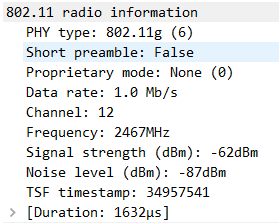
\includegraphics[width=8cm]{parte1global.PNG}
\caption{Informação geral da trama escolhida: 365}
\end{figure}


\subsection*{Questão 1}
\hspace{3mm} 
\questionE{Identifique em que frequência do espectro está a operar a rede sem fios, e o canal que corresponde essa frequência.}\\ 

A rede sem fios está a operar nos 2467 MHz, ou seja, no espectro dos 2 GHz. O canal que está a ser usado é o 12.

\begin{figure}[H]
\begin{center}
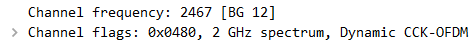
\includegraphics[width=12cm]{1.PNG}
\end{center}
\caption{Frequência e canal da operação}
\end{figure}

\begin{figure}[H]
\begin{center}
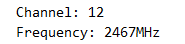
\includegraphics[width=6cm]{1a.PNG}
\end{center}
\caption{Frequência e canal da operação}
\end{figure}

\clearpage

\subsection*{Questão 2}
\hspace{3mm} 
\questionE{Identifique a versão da norma IEEE 802.11 que está a ser usada.}\\ 

A versão que está a ser utilizada é a IEEE 802.11g.

\begin{figure}[H]
\begin{center}
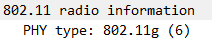
\includegraphics[width=7cm]{2.PNG}
\end{center}
\caption{Versão da norma utilizada}
\end{figure}

\subsection*{Questão 3}
\hspace{3mm} 
\questionE{Qual o débito a que foi enviada a trama escolhida? Será que esse débito corresponde ao débito máximo a que a interface WiFi pode operar? Justifique.}\\ 

Uma vez que está a ser usada a versão IEEE 802.11g, esperam-se débitos até 54 Mbps. No entanto, a trama escolhida, de acordo com a figura 4, foi transmitida a 1.0 Mb/s.

São vários os fatores que impossibilitam uma trama de ser transmitida no débito máximo, como as interferências com máquinas a operar na mesma frequência, obstáculos, redes vizinhas... mas, o principal, acaba por ser, invariavelmente, a distância do host ao AP. Tal facto leva a que o sinal seja menor, implicando um BER mais alto e, por isso, a transmissão é feita de forma mais lenta porque dessa forma é possível reduzir o BER. Nas redes Wi-Fi, a força do sinal é, de facto, diretamente proporcional à taxa de transferência de dados.

\begin{figure}[H]
\begin{center}
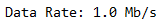
\includegraphics[width=6cm]{3.PNG}
\end{center}
\caption{Débito da trama}
\end{figure}

\clearpage

\section{Scanning Passivo e Scanning Ativo}

\subsection*{Questão 4}
\hspace{3mm} 
\questionE{Selecione uma trama beacon (e.g., a trama 3XX). Esta trama pertence a que tipo de tramas 802.11? Indique o valor dos seus identificadores de tipo e de subtipo. Em que parte concreta do cabeçalho da trama estão especificados (ver anexo)?}\\ 

Escolheu-se a trama 365. Esta trama é do tipo \textit{Management Frame} (id 0) com subtipo \textit{Beacon Frame} (id 8). Os seus identificadores estão especificados no cabeçalho IEEE 802.11 Beacon Frame.

\begin{figure}[H]
\begin{center}
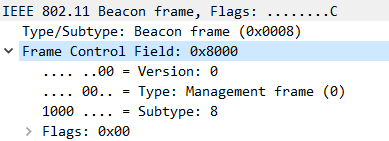
\includegraphics[width=10cm]{4.PNG}
\end{center}
\caption{Identificadores do tipo e subtipo da trama escolhida}
\end{figure}

\clearpage

\subsection*{Questão 5}
\hspace{3mm} 
\questionE{Liste todos os SSIDs dos APs (Access Points) que estão a operar na vizinhança da STA de captura? Explicite o modo como obteve essa informação. Como sugestão pode construir um filtro de visualização apropriado (tomando como base a resposta da alínea anterior) que lhe permita obter a listagem pretendida.}\\ 

Para listar todos os SSIDs presentes na vizinhança, aplicou-se o filtro \texttt{wlan.fc.type\_subtype == 0x0008}. Este filtro possibilita que apareçam só os \textit{Beacon Frames}. Pela análise de todos, verificou-se pelos seus SSIDs que estão duas redes a operar na vizinhança: NOSFON e FlyingNet.

\begin{figure}[H]
\begin{center}
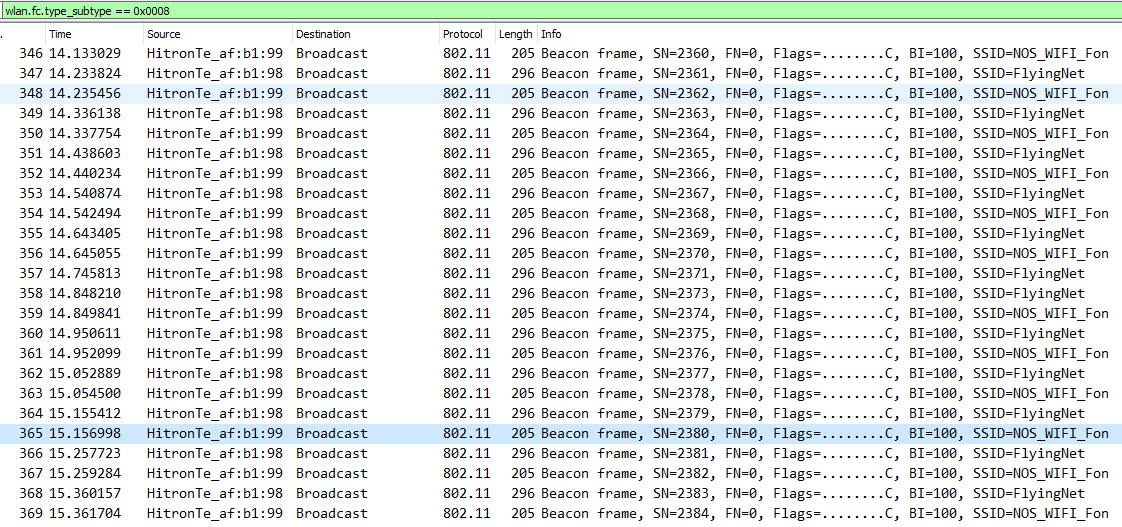
\includegraphics[width=12cm]{5.PNG}
\end{center}
\caption{Beacon Frames das redes vizinhas}
\end{figure}

\subsection*{Questão 6}
\hspace{3mm} 
\questionE{Verifique se está a ser usado o método de detecção de erros (CRC), e se todas as tramas Beacon são recebidas corretamente. Justifique o porquê de usar detecção de erros neste tipo de redes locais.}\\ 

Através da figura 9, podemos verificar que o método de deteção de erros (CRC) está a ser utilizado. Podemos também confirmar, na Figura 8, que nem todas as tramas \textit{Beacon} foram recebidas corretamente, pois todas as assinaladas a azul têm \textit{FCS Status: Bad}.

Nas redes Wi-Fi é quase sempre utilizado o CRC de modo a detetar os erros, pois a maneira de corrigir estes é retransmitir a trama onde o erro ocorreu. Contrariamente a uma rede Ethernet, as redes Wi-Fi tem uma maior probabilidade de ocorrência de erros devido a vários fatores, sendo alguns deles, o meio onde é transmitida a informação, a distância entre o AP e o host, interferências de outras máquinas a operar na mesma frequência, etc. 

\begin{figure}[H]
\begin{center}
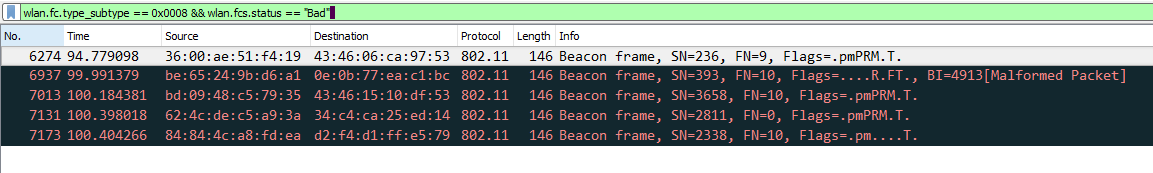
\includegraphics[width=13cm]{6.PNG}
\end{center}
\caption{Uso de um filtro para detetar Bad Packets}
\end{figure}

\begin{figure}[H]
\begin{center}
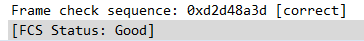
\includegraphics[width=10cm]{6a.PNG}
\end{center}
\caption{Campo de FCS de uma trama}
\end{figure}

\subsection*{Questão 7}
\hspace{3mm} 
\questionE{Para dois dos APs identificados, indique qual é o intervalo de tempo previsto entre tramas beacon consecutivas? (Nota: este valor é anunciado na própria trama beacon). Na prática, a periodicidade de tramas beacon é verificada? Tente explicar porquê.}\\  

O intervalo de tempo previsto é de 0.102400 segundos, como se pode ver na figura 10. Esta periodicidade de tramas \textit{Beacon} não se verifica ao longo do tempo porque assim como todas as outras, têm de obedecer ao algoritmo CSMA/CA. Se existirem tramas a ser transmitidas quando uma nova \textit{Beacon} tem de ser transmitida, então esta espera. Isto leva a uma diferença entre o tempo previsto e o real.

\begin{figure}[H]
\begin{center}
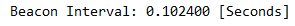
\includegraphics[width=8cm]{7.PNG}
\end{center}
\caption{Intervalo de tempo entre beacons}
\end{figure}

\subsection*{Questão 8}
\hspace{3mm} 
\questionE{Identifique e registe todos os endereços MAC usados nas tramas \textit{Beacon} enviadas pelos APs. Recorde que o endereçamento está definido no cabeçalho das tramas 802.11, podendo ser utilizados até quatro endereços com diferente semântica. Para uma descrição detalhada da estrutura da trama 802.11, consulte o anexo ao enunciado}\\ 

Observa-se o campo BSS Id para identificar os endereços MAC das tramas \textit{Beacons} dos pontos de acesso, embora que, como são \textit{Management Frames}, os campos \textit{Transmitter address}, \textit{Source address} e BSS coincidem.

\begin{itemize}
    \item FlyingNet -> BSS Id = HitronTe\_af:b1:98 (bc:14:01:af:b1:98)
    \item NOS FON -> BSS Id = HitronTe\_af:b1:99 (bc:14:01:af:b1:99)
\end{itemize}

\begin{figure}[H]
\begin{center}
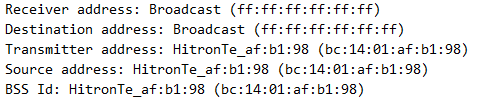
\includegraphics[width=12cm]{8flyingnet.PNG}
\end{center}
\caption{Endereços de beacons enviados pela rede FlyingNet}
\end{figure}

\begin{figure}[H]
\begin{center}
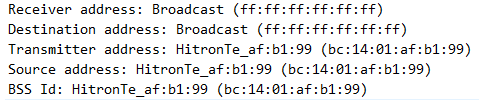
\includegraphics[width=12cm]{8nosfon.PNG}
\end{center}
\caption{Endereços de beacons enviados pela rede NOSFON}
\end{figure}

\subsection*{Questão 9}
\hspace{3mm} 
\questionE{As tramas beacon anunciam que o AP pode suportar vários débitos de base assim como vários “extended supported rates”. Indique quais são esses débitos?}\\ 

Os débitos base suportados do AP são:

\begin{itemize}
    \item 1 Mbit/sec
    \item 2 Mbit/sec
    \item 5.5 Mbit/sec
    \item 11 Mbit/sec
\end{itemize}

Os débitos não base suportados do AP são:

\begin{itemize}
    \item 9 Mbit/sec
    \item 18 Mbit/sec
    \item 36 Mbit/sec
    \item 54 Mbit/sec
\end{itemize}

Os \textit{extended supported rates} base são:

\begin{itemize}
    \item 6 Mbit/sec
    \item 12 Mbit/sec
    \item 24 Mbit/sec
\end{itemize}

O \textit{extended supported rate} não base é:

\begin{itemize}
    \item 48 Mbit/sec 
\end{itemize}

\begin{figure}[H]
\begin{center}
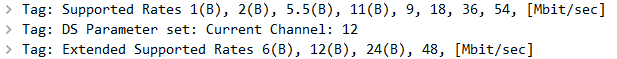
\includegraphics[width=12cm]{9.PNG}
\end{center}
\caption{Débitos do AP}
\end{figure}

\clearpage

\subsection*{Questão 10}
\hspace{3mm} 
\questionE{Estabeleça um filtro Wireshark apropriado que lhe permita visualizar todas as tramas probing request ou probing response, simultaneamente.}\\ 

Filtro utilizado: \textit{wlan.fc.type\_subtype == 5 || wlan.fc.type\_subtype == 4"}.

\begin{figure}[H]
\begin{center}
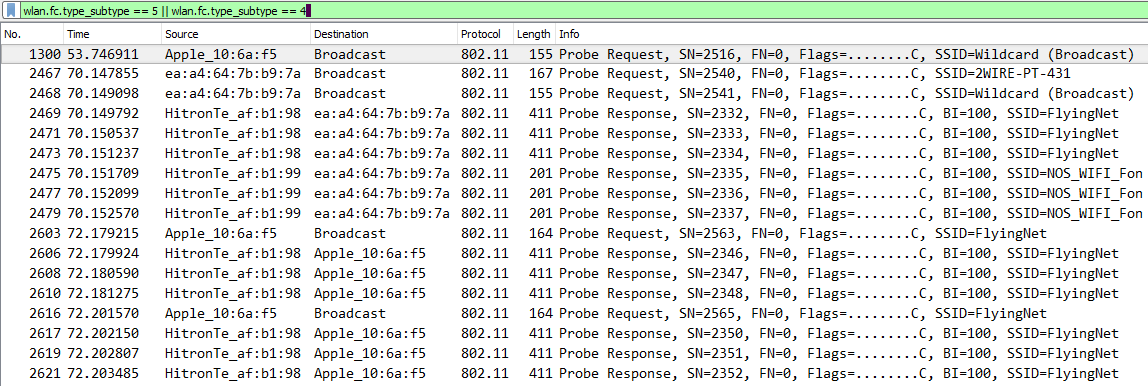
\includegraphics[width=12cm]{10.PNG}
\end{center}
\caption{Filtro para tramas probing request e probing response}
\end{figure}

\subsection*{Questão 11}
\hspace{3mm} 
\questionE{Identifique um probing request para o qual tenha havido um probing response. Face ao endereçamento usado, indique a que sistemas são endereçadas estas tramas e explique qual o propósito das mesmas?}\\

Na trama 2468 identificou-se um \texttt{probing request} que foi direcionado a todos os APs ao alcance do host (ea:a4:64:7b:b9:7a), neste caso FlyingNet e NOSFON. Os \texttt{probing request} são tramas que são usadas quando os hosts querem saber os APs que estão no seu alcance ou quando necessitam de informações de outros hosts.

Imediatamente a seguir, verifica-se uma trama \texttt{probing response}, resposta à trama anterior, enviada pelo AP da FlyingNet.

\begin{figure}[H]
\begin{center}
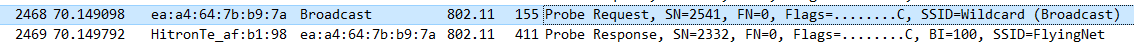
\includegraphics[width=13cm]{11.PNG}
\end{center}
\caption{Probing request e Probing response}
\end{figure}

\begin{figure}[H]
\begin{center}
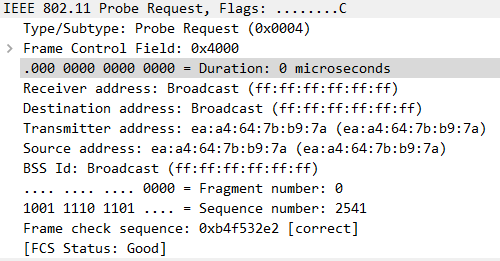
\includegraphics[width=11cm]{11request.PNG}
\end{center}
\caption{Probing request}
\end{figure}

\begin{figure}[H]
\begin{center}
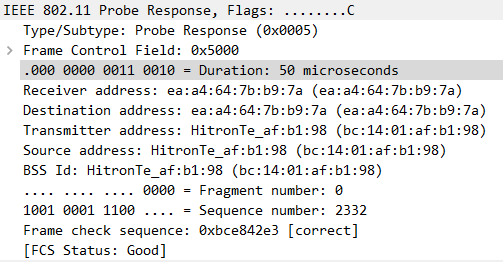
\includegraphics[width=11cm]{11response.PNG}
\end{center}
\caption{Probing response}
\end{figure}

\clearpage

\section{Processo de Associação}

\subsection*{Questão 12}
\hspace{3mm} 
\questionE{Identifique uma sequência de tramas que corresponda a um processo de associação completo entre a STA e o AP, incluindo a fase de autenticação.}\\ 

O processo tem início na trama 2486 e termina na trama 2493. 

\begin{figure}[H]
\begin{center}
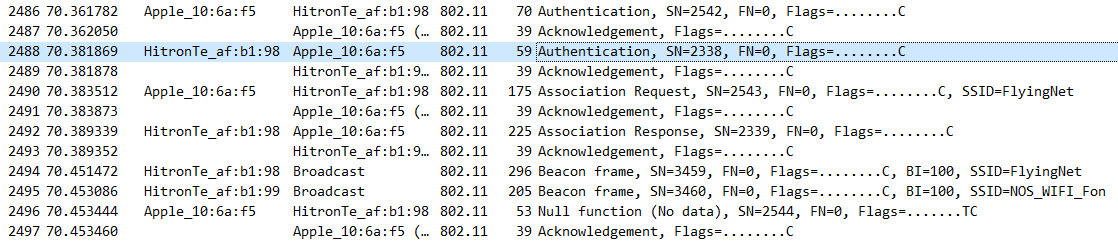
\includegraphics[width=12cm]{12.PNG}
\end{center}
\caption{Processo de associação entre STA e AP}
\end{figure}

\clearpage

\subsection*{Questão 13}
\hspace{3mm} 
\questionE{Efetue um diagrama que ilustre a sequência de todas as tramas trocadas no processo.}\\ 

\begin{figure}[H]
\begin{center}
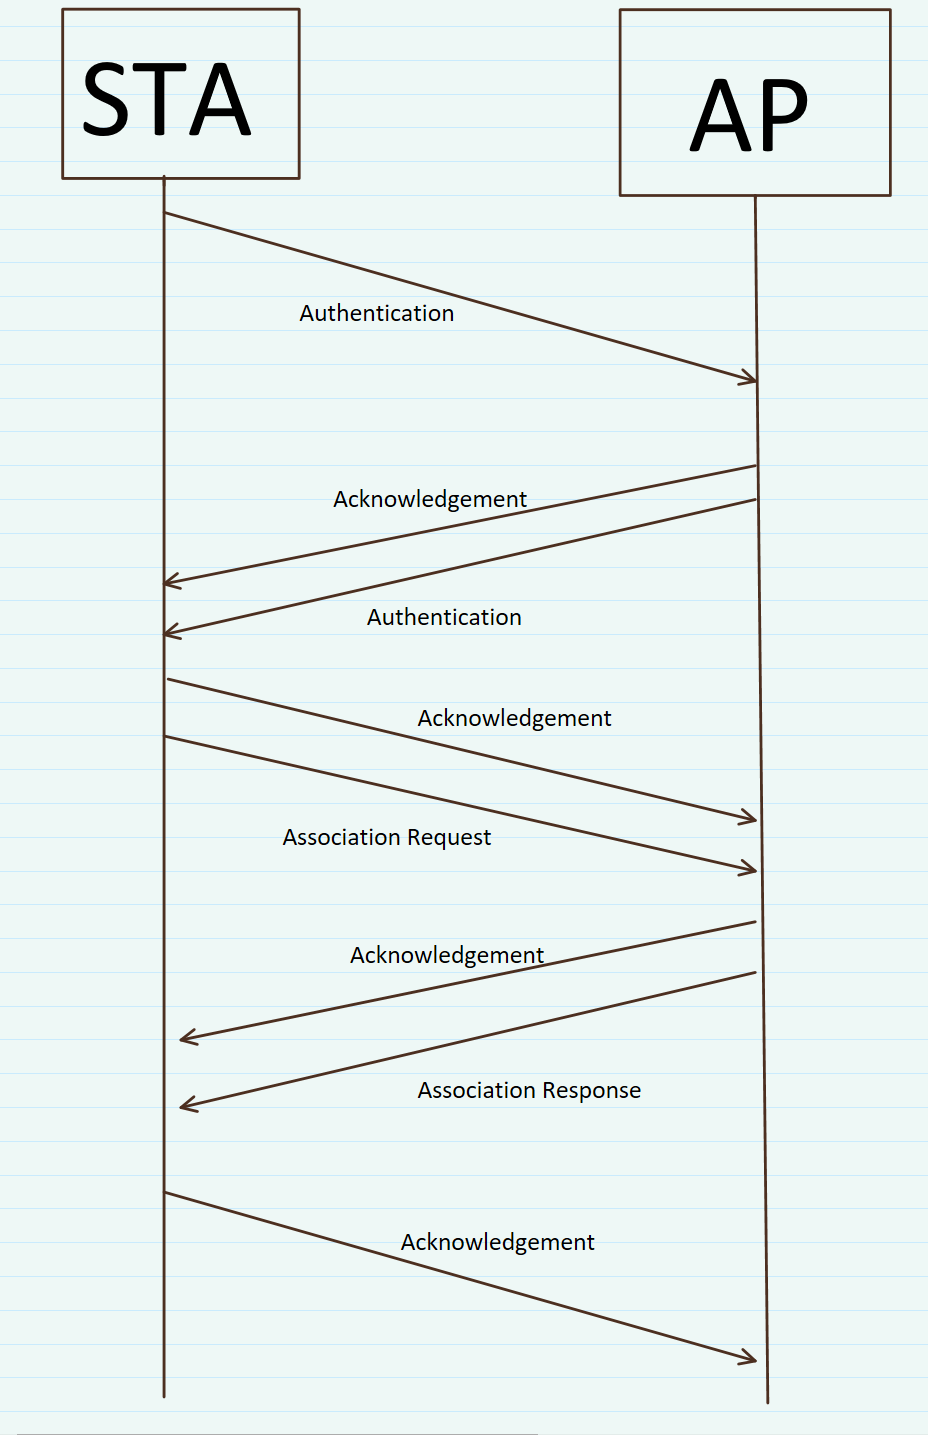
\includegraphics[width=9cm]{ass.PNG}
\end{center}
\caption{Diagrama de sequência das tramas.}
\end{figure}

\clearpage

\section{Transferência de Dados}

\subsection*{Questão 14}
\hspace{3mm} 
\questionE{Considere a trama de dados nº455. Sabendo que o campo Frame Control contido no cabeçalho das tramas 802.11 permite especificar a direccionalidade das tramas, o que pode concluir face à direcionalidade dessa trama, será local à WLAN?}\\ 

O professor, na aula prática, sugeriu que a trama nº455 fosse substituída pela trama nº 818.

A trama tem direção do \textit{Distribution System} para a STA, pois tem o campo \textit{From DS} a 1, o que significa que vem do \textit{Distribution System}. O AP envia, então, a trama para o dispositivo com o MAC Apple\_10:6a:f5. É, por isso, uma comunicação do sistema distribuído para a WLAN local.

\begin{figure}[H]
\begin{center}
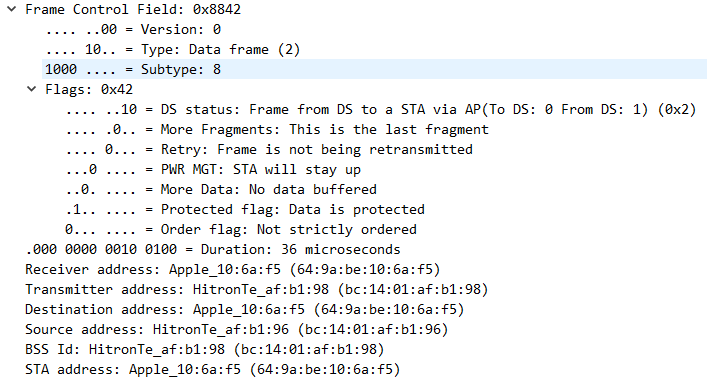
\includegraphics[width=12cm]{14.PNG}
\end{center}
\caption{Direção da trama nº818}
\end{figure}

\subsection*{Questão 15}
\hspace{3mm} 
\questionE{Para a trama de dados nº455, transcreva os endereços MAC em uso, identificando qual o endereço MAC correspondente ao host sem fios (STA), ao AP e ao router de acesso ao sistema de distribuição?}\\ 

Na trama nº455, não se verificou a presença de três endereços diferentes. Deste modo, o professor sugeriu a análise da trama 818.

Na atual situação e tendo em conta as \textit{flags}, verifica-se que o STA address é o endereço do host e o BSS Id é o endereço do AP. Por isso:

\begin{itemize}
    \item Endereço STA: Apple\_71:41:a1 (d8:a2:5e:71:41:a1)
    \item Endereço AP: HitronTe\_af:b1:98 (bc:14:01:af:b1:98)
    \item Endereço Router: HitronTe\_af:b1:96 (bc:14:01:af:b1:96)
\end{itemize}

\begin{figure}[H]
\begin{center}
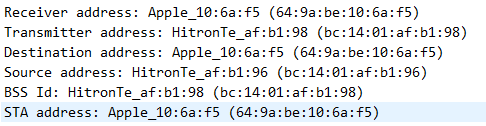
\includegraphics[width=12cm]{15.PNG}
\end{center}
\caption{Endereços da trama nº818}
\end{figure}

\subsection*{Questão 16}
\hspace{3mm} 
\questionE{Como interpreta a trama nº457 face à sua direccionalidade e endereçamento MAC?}\\ 

O professor, na aula prática, sugeriu que a trama nº457 fosse substituída pela trama nº 1434.

A partir das \textit{flags} \texttt{To Ds} e \texttt{From Ds}, é possível verificar a direcionalidade da trama. Neste caso, conclui-se que a direcionalidade é para o sistema distribuído. Aliás, essa é também uma informação que se pode obter a partir dos endereços especificados na figura 22, onde se constata que o endereço origem é a STA e o endereço destino corresponde ao router.

\begin{figure}[H]
\begin{center}
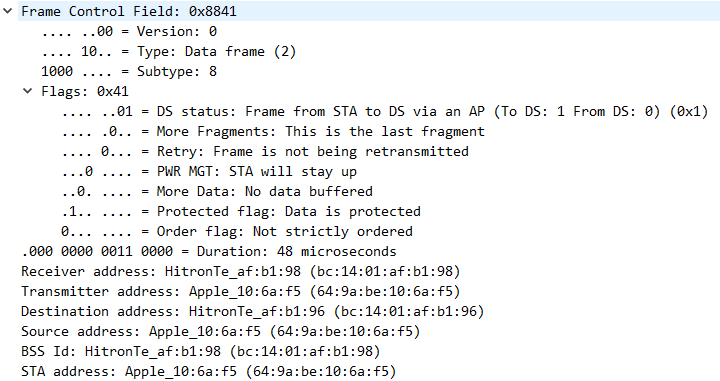
\includegraphics[width=12cm]{16.PNG}
\end{center}
\caption{Frame control da trama nº1434}
\end{figure}

\clearpage

\subsection*{Questão 17}
\hspace{3mm} 
\questionE{Que subtipo de tramas de controlo são transmitidas ao longo da transferência de dados acima mencionada? Tente explicar porque razão têm de existir (contrariamente ao que acontece numa rede Ethernet.)}\\

Estão a ser utilizadas tramas de controlo com o subtipo 1101 que corresponde a tramas \textit{ACK}. Estas tramas são enviadas pelo recetor, logo após a receber a trama, para confirmar a transmissão. Caso esta trama não seja recebida por parte de quem enviou a informação, então a informação volta a ser transmitida. As tramas \textit{ACK} permitem ajudar no \textit{CSMA/CA} \texttt{Carrier-sense multiple access with collision avoidance}, pois é necessário um \textit{ACK} para poder voltar a retransmitir informação na rede.


\begin{figure}[H]
\begin{center}
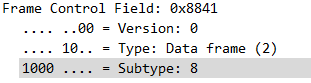
\includegraphics[width=8cm]{17a.PNG}
\end{center}
\caption{Frame Control Field de uma Data Frame}
\end{figure}

\begin{figure}[H]
\begin{center}
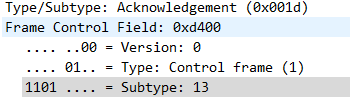
\includegraphics[width=8cm]{17b.PNG}
\end{center}
\caption{Frame Control Field de uma Control Frame}
\end{figure}

\clearpage

\subsection*{Questão 18}
\hspace{3mm} 
\questionE{O uso de tramas Request To Send e Clear To Send, apesar de opcional, é comum para efetuar "pré-reserva" do acesso ao meio quando se pretende enviar tramas de dados, com o intuito de reduzir o número de colisões resultante maioritariamente de STAs escondidas. Para o exemplo acima, verifique se está a ser usada a opção RTS/CTS na troca de dados entre a STA e o AP/Router da WLAN, identificando a direccionalidade das tramas e os sistemas envolvidos.}\\ 

O uso deste tipo de tramas é opcional e verifica-se, principalmente, em situações em que é necessário enviar dados com um tamanho razoável. Por isso, verifica-se na figura 25 que, o STA Apple\_10:6a:f5 envia um \texttt{Request to Send} e obtém resposta \texttt{Clear to Send}. De seguida, há de facto transferência de um volume de dados considerável.

\begin{figure}[H]
\begin{center}
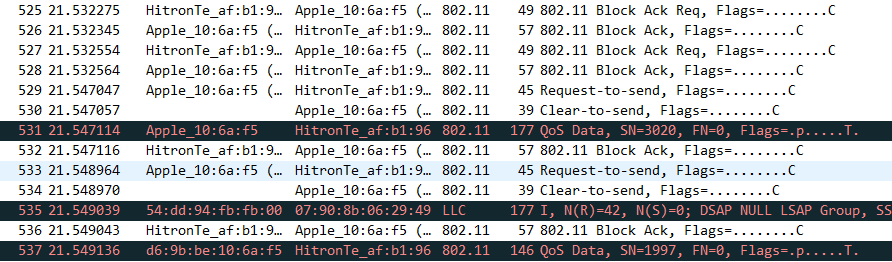
\includegraphics[width=12cm]{18.PNG}
\end{center}
\caption{RTS e CTS entre STA e AP}
\end{figure}

\section{Conclusão}
\hspace{3mm}

Neste trabalho aprofundou-se o conhecimento do funcionamento interno das redes sem fios \texttt{802.11}. Em particular, estudou-se as comunicações entre estações, endereçamento, tipos e sub-tipos de tramas e seu conteúdo.

Consolidou-se o funcionamento e o conceito de deteção de erros e controlo de envio de volumes de dados (RTS e CTS), assim como o de \textit{beacons} e a sua funcionalidade em redes deste tipo. A exploração de \textit{probing} também se tornou relevante para entender comunicação por meio de ar.

Concluiu-se, na realidade, que as redes sem fios são altamente dinâmicas e concorrentes e têm uma complexidade muito mais elevada do que as redes Ethernet.

%BIBLIOGRAFIA


\end{document}